% !TEX TS-program = XeLaTeX
% use the following command:
% all document files must be coded in UTF-8
\documentclass[spanish]{textolivre}
% build HTML with: make4ht -e build.lua -c textolivre.cfg -x -u article "fn-in,svg,pic-align"

\journalname{Texto Livre}
\thevolume{15}
%\thenumber{1} % old template
\theyear{2022}
\receiveddate{\DTMdisplaydate{2021}{9}{10}{-1}} % YYYY MM DD
\accepteddate{\DTMdisplaydate{2021}{10}{14}{-1}}
\publisheddate{\DTMdisplaydate{2021}{11}{26}{-1}}
\corrauthor{Raquel Barragán Sánchez}
\articledoi{10.35699/1983-3652.2022.36032}
%\articleid{NNNN} % if the article ID is not the last 5 numbers of its DOI, provide it using \articleid{} commmand
\runningauthor{Barragán Sánchez et al.} 
%\editorname{Leonardo Araújo} % old template
\sectioneditorname{Daniervelin Pereira}
\layouteditorname{Anna Izabella Pereira}

\title{Autopercepción inicial y nivel de competencia digital del profesorado universitario}
\othertitle{Autopercepção inicial e nível de competência digital de professores universitários}
\othertitle{Initial self-perception and level of digital competence of university teaching staff}
% if there is a third language title, add here:
%\othertitle{Artikelvorlage zur Einreichung beim Texto Livre Journal}

\author[1]{Raquel Barragán Sánchez \orcid{0000-0001-6336-2728} \thanks{Email: \url{rbarragan@us.es}}}
\author[1]{Carmen Llorente Cejudo \orcid{0000-0002-4281-928X} \thanks{Email: \url{karen@us.es}}}
\author[2]{Sonia Aguilar Gavira \orcid{0000-0002-4168-271X} \thanks{Email: \url{sonia.aguilar@uca.es}}}
\author[2]{Remedios Benítez Gavira \orcid{0000-0001-6937-9221} \thanks{Email: \url{r.benitez@uca.es}}}
\affil[1]{Universidad de Sevilla, Facultad de Ciencias de la Educación, Departamento de Didáctica y Organización Educativa, Sevilla, España.}
\affil[2]{Universidad de Cádiz, Facultad de Ciencias de la Educación, Departamento de Didáctica, Cádiz, España.}

\addbibresource{article.bib}
% use biber instead of bibtex
% $ biber article

% used to create dummy text for the template file
\definecolor{dark-gray}{gray}{0.35} % color used to display dummy texts
\usepackage{lipsum}
\SetLipsumParListSurrounders{\colorlet{oldcolor}{.}\color{dark-gray}}{\color{oldcolor}}

% used here only to provide the XeLaTeX and BibTeX logos
\usepackage{hologo}

% if you use multirows in a table, include the multirow package
\usepackage{multirow}

% provides sidewaysfigure environment
\usepackage{rotating}

% CUSTOM EPIGRAPH - BEGIN 
%%% https://tex.stackexchange.com/questions/193178/specific-epigraph-style
\usepackage{epigraph}
\renewcommand\textflush{flushright}
\makeatletter
\newlength\epitextskip
\pretocmd{\@epitext}{\em}{}{}
\apptocmd{\@epitext}{\em}{}{}
\patchcmd{\epigraph}{\@epitext{#1}\\}{\@epitext{#1}\\[\epitextskip]}{}{}
\makeatother
\setlength\epigraphrule{0pt}
\setlength\epitextskip{0.5ex}
\setlength\epigraphwidth{.7\textwidth}
% CUSTOM EPIGRAPH - END

% LANGUAGE - BEGIN
% ARABIC
% for languages that use special fonts, you must provide the typeface that will be used
% \setotherlanguage{arabic}
% \newfontfamily\arabicfont[Script=Arabic]{Amiri}
% \newfontfamily\arabicfontsf[Script=Arabic]{Amiri}
% \newfontfamily\arabicfonttt[Script=Arabic]{Amiri}
%
% in the article, to add arabic text use: \textlang{arabic}{ ... }
%
% RUSSIAN
% for russian text we also need to define fonts with support for Cyrillic script
% \usepackage{fontspec}
% \setotherlanguage{russian}
% \newfontfamily\cyrillicfont{Times New Roman}
% \newfontfamily\cyrillicfontsf{Times New Roman}[Script=Cyrillic]
% \newfontfamily\cyrillicfonttt{Times New Roman}[Script=Cyrillic]
%
% in the text use \begin{russian} ... \end{russian}
% LANGUAGE - END

% EMOJIS - BEGIN
% to use emoticons in your manuscript
% https://stackoverflow.com/questions/190145/how-to-insert-emoticons-in-latex/57076064
% using font Symbola, which has full support
% the font may be downloaded at:
% https://dn-works.com/ufas/
% add to preamble:
% \newfontfamily\Symbola{Symbola}
% in the text use:
% {\Symbola }
% EMOJIS - END

% LABEL REFERENCE TO DESCRIPTIVE LIST - BEGIN
% reference itens in a descriptive list using their labels instead of numbers
% insert the code below in the preambule:
%\makeatletter
%\let\orgdescriptionlabel\descriptionlabel
%\renewcommand*{\descriptionlabel}[1]{%
%  \let\orglabel\label
%  \let\label\@gobble
%  \phantomsection
%  \edef\@currentlabel{#1\unskip}%
%  \let\label\orglabel
%  \orgdescriptionlabel{#1}%
%}
%\makeatother
%
% in your document, use as illustraded here:
%\begin{description}
%  \item[first\label{itm1}] this is only an example;
%  % ...  add more items
%\end{description}
% LABEL REFERENCE TO DESCRIPTIVE LIST - END


% add line numbers for submission
%\usepackage{lineno}
%\linenumbers

\begin{document}
\maketitle

\begin{polyabstract}
\begin{abstract}
El profesorado en nuestro contexto educativo se ha visto sumergido por los avances tecnológicos, provocando cambios en sus funciones, gestión académica y comunicación. Como resultado, se convierten en guías, mediadores, facilitadores y motivadores de procesos de aprendizajes significativos y relevantes. Dicha situación refleja la importancia que asume en la actualidad la competencia digital docente. En el presente artículo se presenta un estudio realizado al profesorado de la Universidad de Cádiz, que tiene como objetivos conocer el perfil tecnológico y nivel competencial digital del profesorado de la universidad, así como la existencia de diferencias significativas en la autopercepción de las competencias digitales docentes según la rama de conocimiento a la que pertenecen. Para ello, se utilizó una metodología \textit{ex post facto} de tipo descriptivo, lo que permite aplicarse una vez que el hecho ya ha sucedido, utilizando como instrumento el cuestionario DigCompEdu Check-in. Entre los resultados obtenidos se puede destacar: la necesidad de aportar una mayor relevancia y apoyo institucional a la formación en competencias digitales docentes, la necesidad de una mayor oferta formativa del profesorado universitario ante la escasa competencia digital docente, También se demuestra que las ramas de conocimiento pueden condicionar el desarrollo de la competencia digital docente en el professorado. El estudio realizado abre camino hacia la posibilidad de contemplar como plan de formación la creación de un entorno formativo que, bajo la arquitectura de t-MOOC ofrezca, de manera gratuita, capacitación del profesorado universitario. 

\keywords{Competencia digital docente \sep Enseñanza superior \sep Formación del profesorado \sep TIC}
\end{abstract}

\begin{portuguese}
\begin{abstract}
Os professores em nosso contexto educacional têm estado submersos pelos avanços tecnológicos, que têm provocado mudanças em suas funções, gestão acadêmica e comunicação. Como resultado, tornam-se guias, mediadores, facilitadores e motivadores de processos de aprendizagem significativos e relevantes. Essa situação reflete a importância que o ensino de competências digitais assume atualmente. O presente artigo apresenta um estudo realizado com o corpo docente da Universidade de Cádiz, cujos objetivos são conhecer o perfil tecnológico e o nível de competência digital do corpo docente universitário, bem como a existência de diferenças significativas na autopercepção das competências digitais do magistério, de acordo com o ramo do conhecimento a que pertencem. Para tanto, foi utilizada uma metodologia descritiva \textit{ex post facto}, que permite sua aplicação uma vez que o evento já tenha ocorrido, utilizando como instrumento o questionário DigCompEdu Check-in. Entre os resultados obtidos, destacam-se: a necessidade de dar maior relevância e suporte institucional à formação em competências pedagógicas digitais, a necessidade de uma maior oferta formativa de docentes universitários face à escassa competência pedagógica digital e o desenvolvimento de competências pedagógicas digitais no corpo docente. O estudo realizado abre caminho à possibilidade de considerar como plano de formação a criação de um ambiente de formação que, no âmbito da arquitetura do t-MOOC, ofereça, gratuitamente, formação para professores universitários.

\keywords{Ensino de competência digital \sep Ensino de nível superior \sep Treinamento de professor \sep TIC}
\end{abstract}
\end{portuguese}

\begin{english}
\begin{abstract}
Teachers in our educational context have been submerged by technological advances,  which have been causing changes in their functions, academic management and communication. As a result, they have become guides, mediators, facilitators and motivators of significant and relevant learning processes. This situation reflects the importance that teaching digital competence currently assumes.  The present article article presents a study carried out with the  professors of the University of Cádiz, whose objectives are to know the technological profile and digital competence level of  these professionals, as well as the existence of significant differences in the self-perception  of their teaching digital skills according to the branch of knowledge to which they belong. For this, an \textit{ex post facto} descriptive methodology was used, which allows it to be applied once the event has already happened, using the DigCompEdu Check-in questionnaire as an instrument. Among the results obtained, the following can be highlighted: the need to provide greater relevance and institutional support to training in digital teaching competencies, the need for a greater training offer for  college professors in the face of scarce digital teaching competence and the development of digital pedagogical/teaching competences among college professor. The study  sheds light on possibility of contemplating as a training plan the creation of a training environment which based on the architecture of t-MOOC, offers, free of charge, training for university teachers.

\keywords{Digital competence teaching \sep Higher education \sep Teacher training \sep ICT}
\end{abstract}
\end{english}
% if there is another abstract, insert it here using the same scheme
\end{polyabstract}

\section{Introducción}\label{sec-intro}
La transformación producida en relación a las TIC ha provocado un choque con respecto al acceso, así como el uso que se hacen de las mismas en los diferentes sectores y espacios sociales. Es por ello que el profesorado debe intentar trasladar al aula dichas competencias que favorezcan la calidad educativa de su alumnado, así como las competencias necesarias para la formación de una ciudadanía implicada en y con la sociedad. El cambio tecnológico producido en los diferentes sectores sociales hace que las competencias digitales del profesorado sean necesarias para los procesos de enseñanza-aprendizaje. Aún no se han realizado ni explotado totalmente las conexiones entre el alumnado y las mismas, así como en los procesos de enseñanza-aprendizaje \cite{oecd2015}. Además, aún siguen sin ser accesibles para todo el alumnado, como muestra \textcite{albapastor2012} “estos recursos, tan prometedores inicialmente para superar barreras físicas y que, cargados de grandes expectativas para las personas con discapacidad, con frecuencia han supuesto nuevas barreras que dificultan el acceso a los estudios y servicios que ofrecen los centros universitarios, profundizando en ocasiones en la denominada brecha digital” (p. 28-29). La normativa actual nos expone que el sistema educativo debe garantizar la igualdad de oportunidades al alumnado desarrollando al máximo sus potencialidades, para ello señala un sistema educativo de calidad, inclusivo y exigente. En la actualidad, como señalan \textcite{trujillo2020} “los posibles escenarios que se diseñen deben cumplir con estos principios para ajustarse no sólo a la ley, sino también a la situación más deseable para nuestros estudiantes y toda la sociedad” (p.6). 

El profesorado, así como la calidad de su docencia, son dos pilares básicos en todo proceso de innovación, donde la incorporación didáctica de las tecnologías en las aulas es un requisito. En su evolución no podemos olvidarnos que  se  han  pasado  por  diferentes  estadios \cite{barroso2010, cabero2014, hernandez-ortega2021, usart2020}.  sin embargo, la educación superior  ha de evolucionar y adaptarse a los cambios que se van produciendo en una sociedad tecnológica y digitalizada como en la que nos encontramos. Ello implica la proliferación de las tecnologías en el proceso educativo, donde el profesorado, como agente clave del cambio, se ha visto sumergido en una imposición tecnológica que ha requerido cambios en sus funciones, gestión académica y comunicación, convirtiéndose en guías, mediadores, facilitadores y motivadores de procesos de aprendizajes significativos y relevantes. Sus metodologías han requerido cambios, y por ende, una adecuada formación del profesorado en competencias digitales se hace inevitable y urgente para poder aprovechar las posibilidades que las TIC nos ofrecen, y así poder garantizar una educación de calidad.

La competencia digital docente (en adelante CDD) es definida como las habilidades, actitudes y conocimientos indispensables en el profesorado, tanto instrumental como metodológica, para facilitar el aprendizaje del alumnado ante la actual sociedad digital \cite{cabero-almenara2016, domingo-coscollola2019, hall2014}, siendo esta “holística, situada, orientada hacia roles de desempeño, función y relación, sistémica, entrenable y en constante desarrollo” \cite[p. 14]{castaneda2018}. Hablamos de la capacidad de poner en práctica esas habilidades y conocimientos TIC en cualquier situación, de forma que la persona pueda dar respuesta a un objetivo o necesidad existente. Por su parte, \textcite{lazaro2015} la definen como la capacidad que dispone el profesorado y que le permite utilizar las tecnologías con eficacia, de forma adecuada, ajustada a sus discentes y a los aprendizajes que éstos deben alcanzar, creando un contexto enriquecido por la tecnología. Un profesorado alfabetizado digitalmente requiere de habilidades no solo para consumir, compartir y producir la información, sino para poder ser crítico/a y reflexivo/a con la misma, conociendo los elementos relacionados con la ciudadanía digital, siendo esta además de un recurso instrumental un elemento de transformación \cite{garcia2017}. Autoress como \textcite{fraser2013} manifiestan que existen tres etapas por las que cualquier centro educativo y su profesorado debe pasar para favorecer la consecución de dichas competencias digitales, como: 1) investigar y conocer qué significa ser competente digital; 2)  identificar los  niveles  de  competencia  según  la  percepción de  los  propios  docentes, y por último; 3) el  apoyo necesario desde las instituciones para facilitar su formación y garantizar su desarrollo  profesional  como docente.

Disponer de dicha CDD permite al profesorado hacer un uso didáctico de las tecnologías, ser capaz de diseñar espacios de aprendizaje donde el alumnado pueda construir de forma activa sus conocimientos por sí mismo y junto a otras personas, hacer un uso de las tecnologías ajustadas al contexto, las necesidades, inquietudes, promoviendo las capacidades y estilos de aprendizaje de cada estudiante, así como el fomento de la autoestima, confianza e iniciativa por parte del alumnado para participar. Supone una mayor flexibilidad en cuanto al qué, el dónde, el cuándo y el cómo aprender, haciendo un uso de las tecnologías para mejorar y transformar su práctica educativa y enriqueciendo su propio desarrollo profesional. De acuerdo con \textcite{barroso2019} supone “una conversión del papel docente, abandonándose como eje vertebrador de la información y el conocimiento y donde la adquisición de unas competencias pedagógicas adquiere igual o mayor importancia que la tecnológica” (p.139). El modelo TPACK (Technological Pedagogical Content Knowledge) ofrecido por \textcite{koehler2008} ofrece los tipos de conocimiento (disciplinar, pedagógico y tecnológico) que todo profesorado debe dominar e interrelacionar para garantizar una integración de las TIC exitosa en el proceso educativo. Dichos conocimientos, aunque relevantes para la profesionalidad docente, en la actualidad, se consideran insuficientes, pues estas deben ser construidas y generadas también por el alumnado, produciéndose un aprendizaje en cascada.

Diversos organismos internacionales han ofrecido diversas propuestas en relación a los conocimientos y habilidades que el profesorado con CDD debería manejar, entre ellos, el marco común europeo DigCompEdu. Dicho marco, con el objetivo de avanzar y mejorar las investigaciones realizadas hasta el momento establece una serie de áreas a tener en cuenta para incorporar las TIC en la educación por parte de los equipos docentes, como son: compromiso profesional, recursos digitales, enseñanza y aprendizaje, evaluación y retroalimentación, empoderamiento de los estudiantes, y facilitarles una competencia digital que les permita desarrollarse  tanto personal, como social y profesionalmente de forma autónoma a través de los recursos tecnológicos \cite{cabero-almenara2020, colas-bravo2019}.

En relación a las competencias digitales a desarrollar en el alumnado, podemos comprobar según los resultados alcanzados en otras investigaciones, que el nivel o dominio existente es también insuficiente \cite{fernandez-marquez2018, giron2019, paredes2015, sancho-gil2015, sierra_llorente2018, fardoun2020, cao2020, ordonez2021, romero-tena2021} %(Fernández-Marquez, Leiva-Olivenza y López-Meneses, 2018; Girón-Escudero, Cózar-Gutiérrez y González-Calero, 2019; Paredes, Guitert y Rubia, 2015; Sancho-Gil, Bosco, Alonso y Sánchez, 2015; Sierra-Llorente et al., 2018 Fardoun et al. 2020; Cao et al. 2020; Ordoñez-Olmedo et al. 2021: Romero-Tena et al. 2021
, prevaleciendo una brecha en la formación inicial de los futuros docentes en materia tecnológica para podar dar respuesta a las actuales y futuras competencias profesionales como docentes con respecto a su alumnado y como ciudadanos digitales (autónomos, críticos, colaborativos, cooperativos, capaz de desarrollar hábitos y actitudes para aprender a aprender a lo largo de su vida, adaptarse o innovar). La universidad, como agente facilitador, tiene el reto de transferir y aplicar en sus planes de estudios, desde la práctica, todas y cada una de estas competencias digitales descritas desde un punto de vista teórico, pues en gran parte de las aulas el profesorado utiliza las TIC como recurso para planificar su enseñanza, pero en menor medida son utilizadas como medio a través del cual crear espacios que enriquezcan el aprendizaje \cite{almerich2011}. Para ello, es necesaria una planificación del proceso de enseñanza- aprendizaje desde los contenidos curriculares, apostando por su dinamismo, interactividad y ajustados a una comunidad educativa diversa. Ello implica hacer conexiones con el tema, asegurarse de que tienen conocimientos sobre el mismo, aprender a discriminar la abrumadora información a la que tienen acceso. En ello, el/la docente debe orientar y motivar para que el alumnado encuentre respuestas a las inquietudes que tienen con respecto a dicho tema, disponiendo de las herramientas y espacios necesarios para su consecución.

Así mismo, para analizar y valorar las competencias que posee el profesorado se realiza una clasificación de las mismas en siete niveles diferentes, pudiendo ser movibles a lo largo del desarrollo profesional, en función del contexto personal, profesional o las características de la propia persona y que puede favorecer o repercutir en la motivación, iniciativa o propósito del profesorado en el desarrollo de las mismas. Los niveles establecidos son: a) los novatos: los cuales se puede decir que apenas utilizan las tecnologías por lo que requeriría una mayor ayuda para su aplicación; b) los exploradores: quienes han comenzado a experimentar con ellas aunque no disponen aún de estrategias y necesitan mejorar sus competencias; c) los integradores; experimentan con herramientas con objetivos diversos, haciendo uso de estrategias digitales en función del contexto; d) los expertos: tienen seguridad para utilizar las herramientas, evaluando el uso que hace de ellas con el objetivo de mejorar su práctica educativa; e) líderes: disponen de un amplio repertorio de estrategias digitales flexibles, completas y eficaces y ejemplos para otros docentes, y; f) los pioneros: suelen cuestionar las prácticas digitales y pedagógicas contemporáneas, suelen innovar constantemente de las que ellos mismos son líderes y son un modelo a seguir para el profesorado más jóven. Como se ha explicado con anterioridad estos niveles no son estancos, sino que están en continuo movimiento, ya que es posible cambiar de nivel tanto de forma ascendente como descendente en diferentes momentos y contextos. Las tecnologías evolucionan con mucha rapidez, por lo que si no existe una formación permanente en las mismas el profesorado definido como pionero puede dejar de serlo, de la misma forma el profesorado novato puede llegar a ser pionero.

En todo ello, la autopercepción que tiene el profesorado sobre sus competencias es de vital importancia.  Investigaciones en relación a la autopercepción docente universitaria aportan que necesitan formarse con respecto a las transformaciones que se van produciendo en el contexto sociolaboral siendo conscientes de sus necesidades formativas y manifestando el deseo de superarlas \cite{mas-torello2016}. Desde la visión del profesorado universitario \cite{domingo-coscollola2019}, algunas de las principales necesidades en la práctica con respecto a su CDD, son; conectar la universidad con la escuela y la sociedad para poder construir conocimientos con sentido, necesarios para planificar aplicando las tecnologías de forma adecuada, siendo conocedores del porqué y para qué de su uso con el alumnado, un mayor conocimiento en la utilización de comunidades virtuales, que les permita compartir y ampliar sus conocimientos junto a otros usuarios, formación en metodologías activas a través de las tecnologías, donde el alumnado posea un mayor protagonismo y sea capaz de gestionar su aprendizaje, mayor formación crítica para seleccionar las herramientas que mejor se ajusten a los contenidos, necesidades o incluso clima existente en cada momento, prevalencia de conocimiento pedagógico-didáctico de las herramientas que permitan al alumnado construir aprendizajes ante conocimientos instrumentales o utilizar en la universidad herramientas a través de las cuales se le haga habitual el compartir, trabajar el equipo, cooperar.

Ser consciente de sus necesidades y limitaciones hace evidente su necesidad de formación y como muestran \textcite{trujillo2020} “esperamos que, en este momento de incertidumbre, todos trabajemos con un único objetivo en mente: garantizar el desarrollo integral y el bienestar de nuestro alumnado a pesar de las condiciones de pandemia y confinamiento en las cuales vivimos, enseñamos y aprendemos en estos momentos” (p.28).

\subsection{Objetivos de investigación}
Los objetivos de esta investigación son explorar el perfil tecnológico de los docentes objeto de estudio (O1) y conocer el nivel competencial digital del profesorado (O2). Además, se tratará de comprobar si existen diferencias significativas en la autopercepción de la CDD según la rama de conocimiento a la que pertenecen los docentes (O3). Esta información es de gran interés a la hora de diseñar planes formativos para el profesorado universitario ajustados a sus necesidades formativas.

\section{Material y métodos}
Para la realización del presente trabajo, se decidió optar por realizar una investigación de metodología \textit{ex post facto}, entendiéndose por ésta la que permite aplicarse una vez que el hecho ya ha sucedido, sin la necesidad de modificar las diferentes variables que configuran el estudio, tal como apuntan \textcite{hernandez2014}. Para el estudio, se diseñó una investigación de corte transversal, a través del denominado enfoque de investigación descriptivo y contraste de hipótesis, teniendo en cuenta que los participantes del estudio lo conformaban concretamente el profesorado de la Universidad de Cádiz (Andalucía, España). 

\subsection{Población y Muestra}
En la Universidad de Cádiz hay una población de 1634 profesores/as. Para determinar el número necesario de participantes en el estudio, se ha realizado un muestreo aleatorio o probabilístico, enviando la encuesta a todo el profesorado. Según la fórmula de muestras finitas propuesta por \textcite[p. 226]{sierra1988}, calculamos el número de profesores necesarios para obtener una muestra con un nivel de confianza del 95\%, n=312. Finalmente, nuestra muestra está compuesta por 552 docentes siendo muy superior a la requerida. Se ha calculado el error muestral dando como resultado un 3,4 margen que se considera muy adecuado a la población de estudio.

Los participantes en la investigación fueron un total de 552 docentes, de los cuales 292 eran mujeres (52,9\%) y 260 hombres (47,1\%). Del total de la muestra, se establecieron diferentes categorías en cuanto a la pertenencia a las diferentes ramas de conocimiento (\Cref{fig1}); así pues, el 16,7\% (n=92) pertenecían a Artes y Humanidades, el 21,7\% (n= 120) a Ciencias, 13\% (n= 72) a Ciencias de la Salud, 21,7\% (n=120) a Ingeniería y Arquitectura, y el 26,8\% (n= 148) a Ciencias Sociales y Jurídicas.

\begin{figure}[htbp]
 \centering
 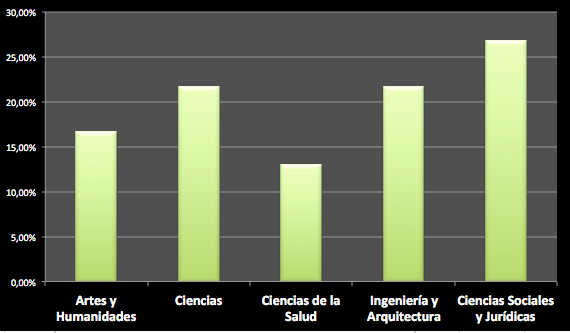
\includegraphics[width=0.6\textwidth]{fig1-36032.png}
 \caption{Pertenencia del profesorado universitarios a las diferentes ramas de conocimiento.}
 \label{fig1}
\source{Elaboración propia.}
\end{figure}

En cuanto a la edad del profesorado, se puede observar que el rango con una menor frecuencia de aparición correspondía a aquellas que oscila entre “25-29 años” (f=16; \%=2,9), y que el que obtuvo una mayor frecuencia de aparición fue el que estaba determinado entre “50-59 años” (f=236; \%=42,8).

Por otro lado, y teniendo en cuenta que posteriormente se realizaron análisis de contraste entre diferentes variables, el trabajo prestó especial atención a los años de experiencia docente del profesorado. En este sentido, y tal como se puede observar en la \Cref{tab1}, varían entre 1 y más de 20 años, donde la frecuencia de aparición mayor estuvo comprendida en el rango de “20 o más años” (48,6\%).

\begin{table}[htpb]
\caption{Experiencia profesional como docente universitario.}
\label{tab1}
\centering
\begin{tabular}{lll}
\toprule
Años de experiencia docente & F & \%
\\ 
\midrule
1-3 años & 52 & 9,4
\\
4-5 años & 32 & 5,8
\\
6-9 años & 68 & 12,3
\\
10-14 años & 64 & 11,6
\\
15-19 años & 68 & 12,3
\\
20 o más años & 268 & 48,6
\\ 
\bottomrule
\end{tabular}
\source{Elaboración propia.}
%\notes{Esta é uma nota exemplo que poderá, opcionalmente, ser adicionada a uma tabela ou figura.}
\end{table}

\subsection{Instrumento y procedimiento de recogida de datos}
Para la recogida de datos del estudio que se presenta se empleó el instrumento denominado “DigCompEdu Check-in”, el cual ha sido empleado en diferentes estudios e investigaciones \cite{cabero-almenara2020, romero-tena2020} y que fue validado por \textcite{ghomi2019} como instrumento a utilizar para el análisis del Marco Europeo de Competencia Digital Docente DigCompEdu. El cuestionario estaba configurado por 6 grandes áreas competenciales: 

A. Compromiso profesional; B. Recursos digitales; C. Pedagogía digital; D. Evaluación y retroalimentación; E. Empoderar a los estudiantes; y F. Facilitar la competencia digital de los estudiantes. 

Las autorías del modelo establecen en estas áreas que, por ejemplo, la primera de ellas (Compromiso profesional) hace alusión a la competencia profesional del docente, y por otro lado, el resto de ellas, están vinculadas más directamente a la competencia digital del alumnado. 

De estas seis grandes áreas, el cuestionario se estructura en un total de 22 ítems que son los que el profesorado cumplimenta de manera online a través de la plataforma “EuSurvey”, y cuya recogida de datos en el estudio que se presenta, se lleva a cabo durante los meses de enero y febrero del año 2020. 

Cabe recordar que el modelo, a través de los diferentes ítems, mide las competencias digitales que conforman el marco competencial, y que queda estructurado en tres grandes bloques: 

\begin{itemize}
    \item A1. Comunicación organizacional; A2. Colaboración profesional; A3. Práctica Reflexiva; A4. Desarrollo profesional continuo. 
    \item B1. Selección de recursos digitales; B2. Creación y modificación de recursos digitales; B3. Administrar, proteger y compartir recursos digitales. 
    \item C1. Enseñanza; C2. Guía; C3. Aprendizaje colaborativo; C4. Aprendizaje autodirigido.
    \item D1. Estrategias de evaluación; D2. Analizar pruebas; D3. Retroalimentación y planificación.
    \item E1. Accesibilidad e inclusión; E2. Diferenciación y personalización; E3. Participación activa de los estudiantes. 
    \item F1. Información y alfabetización mediática; F2. Comunicación y colaboración digital; F3. Creación de contenido digital; F4. Bienestar; F5. Solución digital de problemas.
\end{itemize}

Para analizar los resultados obtenidos antes y después de aplicar el cuestionario, se le pide al profesorado que se autocalifique cómo de competente digital se autopercibe. Con ello permite realizar un pre-post test a la hora de establecer las diferentes categorías de experticia en el uso de las TIC, y que clasifican en: A1 “Novato”, A2 “Explorador”, B1 “Integrador”, B2 “Experto”, C1 “Líder” y C2 “Pionero”. El cuestionario se puede consultar completo en el \Cref{anex1}.

Para la fiabilización del cuestionario, y aunque el instrumento está validado ya con anterioridad a través de diferentes métodos (Barragán-Sánchez, Llorente-Cejudo, Puig-Gutiérrez y Romero-Tena, 2020; Cabero-Almenara, Barroso-Osuna, Palacios-Rodríguez y Llorente-Cejudo, 2020), en el estudio que se presenta, se aplicó el Alfa de Cronbach (\Cref{tab2}) para obtener el índice de consistencia interna del instrumento, obteniendo los resultados que se presentan a continuación. 

\begin{table}[htpb]
\caption{Estadístico de fiabilidad. Alfa de Cronbach.}
\label{tab2}
\centering
\begin{tabular}{ll}
\toprule
Alfa de Cronbach & Número de elementos
\\ 
\midrule
,923 & 22
\\ 
\bottomrule
\end{tabular}
\source{Elaboración propia.}
\end{table}

Como puede observarse, una puntuación de 0,923 muestra una significatividad alta que, de acuerdo con \textcite[p. 189]{bisquerra1987} indica que correlaciones situadas entre el intervalo 0.8 y 1 pueden considerarse como “muy altas” y, en consecuencia, denotarían unos altos niveles de fiabilidad del instrumento.  

\subsection{Análisis de los datos}
Los análisis que se aplican son, frecuencias, porcentajes y medidas de tendencia central (media) y dispersión (desviación estándar). Además, se emplean estadísticos de contraste para comprobar la significatividad de las diferencias entre las percepciones competenciales de los docentes y las ramas de conocimiento a la que pertenecen. En concreto, se aplica el estadístico no paramétrico Prueba de Kruskal-Wallis. Paralelamente, se ha comprobado que los datos no se distribuyen normalmente a través del estudio de asimetría y curtosis. La prueba de “bondad de ajuste Kolmogorov-Smirnov” ha confirmado esta comprobación, con significación (p-valor) igual a .000 para todos los ítems (distribución no normal). En todo momento, los datos obtenidos son analizados con el paquete estadístico SPSS (V.26).

\section{Resultados}
\subsection{Perfil tecnológico}
En lo que respecta al perfil tecnológico, lo hemos medido mediante el tiempo de uso que los docentes dedican a las TIC, el tiempo dedicado a la tecnología en el aula, la autopercepción y dominio de distintas tecnologías como ordenador, tablet, smartphone e Internet y el uso de redes sociales (O1).

En lo que respecta al tiempo que los docentes universitarios manifiestan que emplean y dedican a las TIC, los resultados se pueden observar en la \Cref{tab3}.

\begin{table}[htpb]
\caption{Tiempo de uso de las TIC por el profesorado universitario.}
\label{tab3}
\centering
\begin{tabular}{p{0.4\textwidth}p{0.05\textwidth}p{0.05\textwidth}}
\toprule
Tiempo uso de las tecnologías & F & \%
\\ 
\midrule
No uso la tecnología como herramienta educativa & 4 & ,7
\\
Menos de 1 año & 4 & ,7
\\
1-3 años & 68 & 12,3
\\
4-5 años & 44 & 8,0
\\
6-9 años & 72 & 13,0
\\
10-14 años & 180 & 32,6
\\
15-19 años & 96 & 17,4
\\
20 años o más & 84 & 15,2
\\ 
\bottomrule
\end{tabular}
\source{Elaboración propia.}
\end{table}

La mayoría del profesorado universitario preguntado en el estudio, manifestó que llevaban alrededor de 10 a 14 años usando las tecnologías (f=180; 32,6\%), seguida de 15-19 años (f=96; 17,4\%) y, en menor medida de aparición, los intervalos de “Menos de 1 año” y “No uso la tecnología como herramienta educativa”, obtenido los dos la misma frecuencia y porcentaje de aparición (f=4; 0.7\%). 

Por último, en estas primeras variables de análisis, se les preguntó al profesorado por el porcentaje de tiempo dedicado al uso de la tecnología (\Cref{tab4}), pero esta vez más concretamente, en el ámbito de clase y no de manera general o de ocio. Así pues, los resultados se presentan a continuación. 

\begin{table}[htpb]
\caption{Tiempo dedicado al uso de la tecnología en clase.}
\label{tab4}
\centering
\begin{tabular}{p{0.3\textwidth}p{0.05\textwidth}p{0.05\textwidth}}
\toprule
Porcentaje de tiempo dedicado al uso de la tecnología en clase & F & \%
\\ 
\midrule
0-10\% & 28 & 5,1
\\
11-25\% & 116 & 21,0
\\
26-50\% & 204 & 37,0
\\
51-75\% & 124 & 22,5
\\
76-100\% & 80 & 14,5
\\ 
\bottomrule
\end{tabular}
\source{Elaboración propia.}
\end{table}

Los datos muestran como existe una mayor parte de los encuestados que manifiestan que hacen un tiempo elevado en el uso de las TIC como herramienta educativa.

En lo que respecta a la cuestión sobre cómo de competentes se sienten para el manejo de las diferentes tecnologías, es decir, su dominio tecnológico, los resultados obtenidos se presentan en la siguiente \Cref{tab5}. 

\begin{table}[htpb]
\caption{Competencias en el manejo de diferentes tecnologías.}
\label{tab5}
\centering
\begin{tabular}{p{0.13\textwidth}p{0.13\textwidth}p{0.13\textwidth}p{0.13\textwidth}p{0.13\textwidth}p{0.13\textwidth}}
\toprule
\multicolumn{6}{l}{En mi día a día se manejar…}
\\
\midrule
Medio & Totalmente en desacuerdo & En desacuerdo & Ni desacuerdo\/Ni de acuerdo & De acuerdo & Muy de acuerdo
\\ 
\midrule
Ordenador & - & 36 (6,5\%) & - & 3468 (12\%) & 448 (81\%)
\\
Tablet & - & 40 (7,2\%) & 24 (4,3\%) & 104 (18,8\%) & 384 (69,6\%)
\\
Smartphone & - & 36 (6,5\%) & 24 (4,3\%) & 96 (17,4\%) & 396 (71,7\%)
\\
Internet & 36 (6,5\%) & - & 16 (2,9\%) & 112 (20,3\%) & 388 (70,3\%)
\\ 
\bottomrule
\end{tabular}
\source{Elaboración propia.}
\end{table}

Los datos muestran cómo, de manera global, la gran mayoría del profesorado encuestado mostraban una actitud favorable hacia el manejo de las tecnologías, recursos, aplicaciones y programas. Más concretamente, el ordenador fue el medio con el que se sienten más competentes en el manejo en su uso diario, donde el 81\% manifestaba estar muy de acuerdo (n=448), seguido del Smartphone con un 71,7\% (n=396) de respuestas obtenidas. En este sentido, se puede comprobar como la mayoría de respuesta obtenidas en los diferentes medios analizados (Ordenador, Tablet, Smartphone o Internet) hacían alusión a que el profesorado se sentía muy de acuerdo en la competencia hacia el uso de dichas tecnologías en su día a día. 

Por último, también se quiso conocer el número de redes a las que el profesorado se encontraban suscritos. Cabe decir que, la mayoría manifestaron estar suscritos a un total de 3 redes sociales (f=140; \%25,4), y que sólo el 6,5\% (n=36) apuntaban que lo estaban a más de 6 redes sociales.

\subsection{Análisis competencial}
A continuación, se presentan los datos referentes a las percepciones del profesorado sobre sus competencias digitales (O2).

En la \Cref{tab6} se muestran los resultados de la autopercepción de las competencias por parte del profesorado universitario. La escala en la que se miden cada una de las competencias se presentan en una medida entre 0 y 4. 

\begin{longtable}{p{0.8\textwidth}p{0.05\textwidth}p{0.05\textwidth}}
%\begin{table}[htpb]
\caption{Puntuaciones medias y desviación de las áreas competenciales y competencias que se miden en el cuestionario.}
\label{tab6}
%\begin{tabular}{p{0.8\textwidth}p{0.05\textwidth}p{0.05\textwidth}}
\\
\toprule
& $\tilde{X}$ & $\sigma$
\\ 
\midrule
Área 1: Compromiso Profesional (A) & 2,38 & 0,652
\\
A1. Uso sistemáticamente diferentes canales digitales para mejorar la comunicación con el alumnado y mis compañeros/as. Por ejemplo: correos electrónicos, aplicaciones de mensajería tipo Whatsapp, blogs, el sitio web de la facultad… & 2,40 & ,655
\\
A2. Uso tecnologías digitales para trabajar con mis compañeros/as dentro y fuera de mi organización educativa. & 2,21 & ,983
\\
A3. Desarrollo activamente mi competencia digital docente. & 2,30 & ,931
\\
A4. Participo en cursos de formación online. Por ejemplo: cursos online de la universidad, MOOCs, webinars… & 2,40 & ,655
\\
\midrule
Área 2: Recursos Digitales (B) & 2,33 & 0,685
\\
B1. Utilizo diferentes sitios de internet (páginas web) y estrategias de búsqueda para encontrar y seleccionar una amplia gama de recursos digitales. & 2,32 & ,957
\\
B2. Creo mis propios recursos digitales y modifico los existentes para adaptarlos a mis necesidades como docente. & 2,49 & ,784
\\
B3. Protejo el contenido sensible de forma segura. Por ejemplo: exámenes, calificaciones, datos personales. & 2,20 & 1,132
\\
\midrule
Área 3: Pedagogía Digital (C) & 2,33 & 1,024
\\
C1. Considero cuidadosamente cómo, cuándo y por qué usar las tecnologías digitales en clase, para garantizar que se aproveche su valor añadido. & 2,15 & 1,051
\\
C2. Superviso las actividades e interacciones de mis alumnos en los entornos de colaboración en línea que utilizamos. & 2,55 & ,980
\\
C3. Cuando mis alumnos trabajan en grupos o equipos, usan tecnologías digitales para adquirir y documentar conocimientos. & 2,54 & 1,093
\\
C4. Uso tecnologías digitales para permitir que los estudiantes planifiquen, documenten y evalúen su aprendizaje por sí mismos. Por ejemplo: pruebas de autoevaluación, portfolio digital, blogs, foros… & 2,10 & ,952
\\
\midrule
Área 4: Evaluación y Retroalimentación (D) & 1,38 & 0,573
\\
D1. Uso estrategias de evaluación digital para monitorizar el progreso de los estudiantes. & 1,96 & ,933
\\
D2. Analizo todos los datos disponibles para identificar al alumnado que necesita apoyo adicional. “Datos” incluye: participación de los estudiantes, desempeño, calificaciones, asistencia, actividades e interacciones sociales en entornos en línea... El “alumnado que necesita apoyo adicional” es: aquel en riesgo de abandono escolar, bajo rendimiento, trastorno de aprendizaje, necesidades específicas de aprendizaje o que carece de habilidades transversales (habilidades sociales, verbales o de estudio). & 1,60 & 1,020
\\
D3. Uso tecnologías digitales para proporcionar retroalimentación (feedback) efectiva. & 1,98 & ,865
\\
\midrule
Área 5: Empoderar a los Estudiantes (E) & 1,92 & 0,983
\\
E1. Cuando propongo tareas digitales, considero y abordo posibles problemas como el acceso igualitario a los dispositivos y recursos digitales; problemas de compatibilidad o nivel bajo de competencia digital del alumnado. & 2,15 & 1,217
\\
E2. Uso tecnologías digitales para ofrecer al alumnado oportunidades de aprendizaje personalizadas. Por ejemplo: asignación de diferentes tareas digitales para abordar las necesidades de aprendizaje individuales, tener en cuenta las preferencias e intereses... & 1,46 & 1,277
\\
E3. Uso tecnologías digitales para que el alumnado participe activamente en clase. & 2,17 & ,987
\\
\midrule
Área 6: Facilitar la Competencia Digital de los Estudiantes (F) & 1,86 & 0,736
\\
F1. Enseño al alumnado cómo evaluar la confiabilidad de la información buscada en línea y a identificar información errónea y/o sesgada. & 1,96 & 1,030
\\
F2. Propongo tareas que requieren que los estudiantes usen medios digitales para comunicarse y colaborar entre sí o con una audiencia externa. & 1,96 & ,937
\\
F3. Propongo tareas que requieren que los estudiantes creen contenido digital. Por ejemplo: videos, audios, fotos, presentaciones, blogs, wikis... & 2,22 & 1,079
\\
F4. Enseño al alumnado cómo comportarse de manera segura y responsable en línea. & 1,25 & 1,017
\\
F5. Animo al alumnado a usar las tecnologías digitales de manera creativa para resolver problemas concretos. Por ejemplo, superar obstáculos o retos emergentes en su proceso de aprendizaje. & 1,93 & ,916
\\ 
\bottomrule
%\end{tabular}
\source{Elaboración propia.}
%\end{table}
\end{longtable}

Los valores medios alcanzados por el profesorado en cada uno de los ítems se distribuyen alrededor del valor 2, lo que señala que dicho profesorado se ha posicionado en un valor central. Esto lleva a señalar que, en general, la percepción que tienen de su dominio en CDD es moderada. Destacan los valores más altos en las competencias vinculadas al área 1, 2 y 3 (Compromiso Profesional, Recursos Digitales y Pedagogía Digital). Las puntuaciones más bajas se asocian a las áreas 4, 5 y 6 (Evaluación y Retroalimentación, Empoderar a los Estudiantes y Facilitar la Competencia Digital de los Estudiantes). Destaca en el área 6 la puntuación más baja (1,25) en el ítem “Enseño al alumnado cómo comportarse de manera segura y responsable en línea”. 

En la \Cref{tab7} se muestran los resultados obtenidos del auto-posicionamiento del profesorado al inicio del cuestionario, y el resultado final sobre su nivel competencial.

\begin{table}[htpb]
\caption{Autovaloración previa y resultado final del nivel competencial del profesorado.}
\label{tab7}
\centering
\begin{tabular}{p{0.2\textwidth}p{0.05\textwidth}p{0.05\textwidth}p{0.05\textwidth}p{0.05\textwidth}}
\toprule
\multirow{2}{=}{Nivel} & \multicolumn{2}{c}{Pre} & \multicolumn{2}{c}{Pos}
\\
& f & \% & f & \%
\\
\midrule
A1 Novato & 8 & 1,4 & 12 & 2,2
\\
A2 Explorador & 80 & 14,5 & 64 & 11,6
\\
B1 Integrador & 276 & 50,0 & 288 & 52,2
\\
B2 Experto & 148 & 26,8 & 156 & 28,3
\\
C1 Líder & 18 & 5,1 & 20 & 3,6
\\
C2 Pionero & 12 & 2,2 & 12 & 2,2
\\ 
\bottomrule
\end{tabular}
%\source{Fonte da tabela.}
\end{table}

Como se puede comprobar, existen diferencias entre lo marcado al inicio y el resultado final. En el nivel A1 Novato se produce un aumento de +4, es decir, finalmente hay más docentes en este nivel de los que al principio se situaban en el mismo. En el nivel B1 Integrador, se produce un aumento respecto al pretest de +12. De igual forma en B2 Experto también se produce un aumento +8. En el sentido contrario, en el nivel A2 Explorador hay una disminución de -14, es decir, en la valoración final existen menos docentes en este nivel. También con una valoración menor encontramos el nivel C1 Líder -8. Finalmente hay que señalar que en el nivel C2 Pionero es el único que se mantiene. 

En la \Cref{tab8} se presentan los resultados obtenidos de la autovaloración competencial de los docentes de cada área, vinculado a la rama de conocimiento a la que pertenecen (los resultados se muestran en una escala de 0-4).

\begin{table}[htpb]
\caption{Autovaloración previa y resultado final del nivel competencial del profesorado.}
\label{tab8}
\centering
\begin{tabular}{p{0.22\textwidth}p{0.04\textwidth}p{0.04\textwidth}p{0.04\textwidth}p{0.04\textwidth}p{0.04\textwidth}p{0.04\textwidth}p{0.04\textwidth}p{0.04\textwidth}p{0.04\textwidth}p{0.04\textwidth}}
\toprule
& \multicolumn{10}{c}{Rama}
\\
& \multicolumn{2}{c}{\rotatebox{90}{\parbox{2.6cm}{Artes y \\ Humanidades}}} & \multicolumn{2}{c}{\rotatebox{90}{\parbox{2.6cm}{Ciencias}}} & \multicolumn{2}{c}{\rotatebox{90}{\parbox{2.6cm}{CC. de la Salud}}} & \multicolumn{2}{c}{\rotatebox{90}{\parbox{2.6cm}{Ingeniería y \\ Arquitectura}}} & \multicolumn{2}{c}{\rotatebox{90}{\parbox{2.6cm}{CC. Sociales y \\ Jurídicas}}}
\\
& $\tilde{X}$ & $\sigma$ & $\tilde{X}$ & $\sigma$ & $\tilde{X}$ & $\sigma$ & $\tilde{X}$ & $\sigma$ & $\tilde{X}$ & $\sigma$
\\
\midrule
P. TOTAL & 2,1 & 0,5 & 1,9 & 0,6 & 2,1 & 0,6 & 2,2 & 1,6 & 2 & 0,5
\\
A. Compromiso Profesional & 2,2 & 0,75 & 2,5 & 2,05 & 2,5 & 0,75 & 2,5 & 0,75 & 2,25 & 0,75
\\
B. Recursos Digitales & 2,3 & 0,6 & 2,3 & 0,6 & 2,3 & 0,6 & 2,3 & 0,6 & 2,3 & 0,6
\\
C. Pedagogía Digital & 2,5 & 2,6 & 2,2 & 0,7 & 2,5 & 1 & 2,5 & 1 & 2,25 & 0,7
\\
D. Evaluación y Retroalimentación & 1,6 & 0,6 & 1,5 & 0,6 & 2 & 0,6 & 2 & 1 & 1,6 & 0,6
\\
E. Empoderar a los Estudiantes & 2,3 & 1 & 1,6 & 0,6 & 2 & 1,3 & 2 & 1 & 2 & 1
\\
F. Facilitar la Competencia Digital de los Estudiantes & 2 & 0,6 & 1,6 & 0,6 & 1,8 & 0,8 & 2,2 & 0,8 & 1,8 & 0,8
\\ 
\bottomrule
\end{tabular}
\source{Elaboración propia.}
\end{table}

\subsection{Análisis de contraste}
Con objeto de analizar si estas diferencias de autovaloración según las ramas de conocimiento significativas (O3), se formulan las siguientes hipótesis: 

Diferencias según la rama de conocimiento:

\begin{itemize}
    \item Hipótesis nula (H0): No existen diferencias significativas entre las valoraciones que realiza el profesorado universitario sobre sus competencias según la rama de conocimiento a la que pertenecen.
    \item Hipótesis alternativa (H1): Existen diferencias significativas entre las valoraciones que realiza el profesorado universitario según la rama de conocimiento a la que pertenecen.
\end{itemize}

Para ello se aplica el estadístico no paramétrico Prueba de Kruskal-Wallis. La \Cref{tab9,tab10} presenta los valores de KW y rango promedio.

\begin{table}[htpb]
\caption{Resultados de Kruskal Wallis Nivel competencial y rama de conocimiento.}
\label{tab9}
\centering
\begin{tabular}{p{0.2\textwidth}p{0.11\textwidth}p{0.05\textwidth}p{0.05\textwidth}p{0.05\textwidth}p{0.05\textwidth}p{0.05\textwidth}p{0.05\textwidth}}
\toprule
& P. TOTAL & A & B & C & D & E & F
\\
\midrule
Chi-cuadrado & 10,425 & 4,374 & 1,615 & 6,442 & 3,193 & 14,527 & 27,150
\\
Gl & 4 & 4 & 4 & 4 & 4 & 4 & 4
\\
Sig. asintótica & ,034 & ,358 & ,806 & ,168 & ,526 & ,006 & ,000
\\
\multicolumn{8}{l}{a. Prueba de Kruskal Wallis}
\\
\multicolumn{8}{l}{b. Variable de agrupación: Rama}
\\ 
\bottomrule
\end{tabular}
\source{Elaboración propia.}
\end{table}

Como se puede observar en la \Cref{tab9}, los resultados de la prueba KW, se puede afirmar con un nivel de confianza del 95\% y 99\% que existen diferencias significativas en la variable global de la competencia digital, así como en las áreas E (Empoderar a los Estudiantes) y F (Facilitar la Competencia Digital de los Estudiantes). Por lo que, según los datos obtenidos, la rama de conocimiento a la que pertenece el profesorado objeto de estudio es un elemento importante para la autovaloración de la CDD en los docentes objeto de estudio. Se podría decir que la rama de conocimiento a la que pertenecen puede condicionar la valoración de la competencia digital.

El análisis de rangos promedio indica que las principales diferencias se producen entre las ramas de Artes y Humanidades (alcanzan las puntuaciones más altas) y las de Ciencias (alcanza las puntuaciones más bajas). Este patrón se mantiene e incluso se acentúa en las áreas E (Empoderar a los Estudiantes) y F (Facilitar la Competencia Digital de los Estudiantes), alcanzado la máxima diferencia en la última.

\begin{table}[htpb]
\caption{Rangos promedio Nivel competencial y rama de conocimiento.}
\label{tab10}
\centering
\begin{tabular}{p{0.3\textwidth}p{0.3\textwidth}p{0.16\textwidth}}
\toprule
Dimensión & Rama & Rango promedio
\\
\midrule
\multirow{6}{=}{P. TOTAL} & Artes y Humanidades & 155,63
\\
& Ciencias & 113,33
\\
& Ciencias de la Salud & 144,28
\\
& Ingeniería y Arquitectura & 152,70
\\
& Ciencias Sociales y Jurídicas & 133,93
\\
& Total & 
\\
\midrule
\multirow{6}{=}{E. Empoderar a los Estudiantes} & Artes y Humanidades & 159,28
\\
& Ciencias & 108,10
\\
& Ciencias de la Salud & 136,72
\\
& Ingeniería y Arquitectura & 154,90
\\
& Ciencias Sociales y Jurídicas & 137,80
\\
& Total &
\\
\midrule
\multirow{6}{=}{F. Facilitar la Competencia Digital de los Estudiantes} & Artes y Humanidades & 162,33
\\
& Ciencias & 95,87
\\
& Ciencias de la Salud & 134,89
\\
& Ingeniería y Arquitectura & 162,67
\\
& Ciencias Sociales y Jurídicas & 140,42
\\
& Total &
\\ 
\bottomrule
\end{tabular}
\source{Elaboración propia.}
\end{table}

\section{Discusión y Conclusiones}
Teniendo en cuenta que el principal objetivo del estudio que se presenta fue explorar el perfil tecnológico del profesorado y conocer su nivel de competencia digital, es posible afirmar que, a pesar de las recomendaciones propuestas por el marco europeo para incluir en todas las etapas educativas las TIC, el profesorado objeto de estudio muestra un nivel competencial digital medio-bajo relativo a cada una de las áreas establecidas, siendo la de menor desarrollo entre dicho colectivo la que hace referencia a una de las nuevas áreas incorporadas y, desde nuestro punto de vista, más significativas en la actualidad; es decir, la vinculada a cómo el desarrollar las competencias digitales en el alumnado. Así pues, y tras los resultados obtenidos, puede afirmarse que existe una brecha formativa entre el profesorado universitario en lo que a competencias digitales se refiere, pues las habilidades y capacidades en materia tecnológica de las que se dispone hacen que el uso que se efectúa de ellas en sus aulas no corresponda con los requisitos exigidos en las diferentes áreas del marco europeo con respecto a las competencias digitales. En este sentido, se presenta interesante planificar una propuesta formativa que permita minimizar la brecha formativa del profesorado universitario en lo que respecta a las competencias digitales, y así lo reflejan los excelentes resultados que acciones de diseño como los TMOOC pueden ofrecer un amplio abanico de posibilidades \cite{cabero-almenara2020, cabero-almenara2021}, o a la luz de diferentes estudios vinculados con este campo y relacionados con los resultados del estudio, se puede considerar que los futuros docentes también deberian formarse em el desarrollo del contenido digital \cite{burgos2021, cebi2020}.Unos resultados que reflejan, evidencian, coinciden y confirman, junto con las diversas investigaciones contrastadas, la necesidad de una mayor formación en el profesorado universitario ante la escasa CDD, así como el desarrollo de las mismas en su propio alumnado \cite{barroso2019, domingo-coscollola2019, fernandez-marquez2018, mueller2008, pinto-santos2020, pozo2019, pozos2018}, a pesar del uso de estas en su práctica educativa de forma habitual.

Teniendo en cuenta la propuesta realizada sobre los objetivos de la investigación que se presenta,, se puede considerar, en primer lugar que, con respecto al objetivo de estudio uno (O1) “explorar el perfil tecnológico de los docentes del estudio”, y al segundo (O2) “conocer el nivel competencial digital del profesorado”, se puede concluir que aunque el profesorado participante afirma llevar de 10 a 14 años usando las tecnologías, y mostraban una actitud favorable hacia el manejo de recursos, aplicaciones y programas, la percepción que tienen de su dominio en lo que respecta a la competencia digital docente es moderada, incluso algunos de los docentes que consideraban tener un nivel de “expertos” o “líderes” al comienzo, evolucionan según su práctica docente, a tener un nivel “integrador”, siendo el nivel más destacado entre los participantes.

Es por ello que, se plantea como necesario resaltar la importancia de la formación universitaria en paralelo a la escuela y a la sociedad, en la que no exista un distanciamiento cognitivo tan marcado como el que aparece en la actualidad. 

En este sentido, y al hilo de la necesidad en lo que respecta a la formación en competencias digitales del profesorado universitario, el estudio realizado abre camino hacia la posibilidad de contemplar como plan de formación la creación de un entorno formativo que, bajo la arquitectura de t-MOOC se ofrezca, de manera gratuita, para la capacitación del profesorado universitario a través de una oferta formativa de diferentes niveles, vinculados al Marco Europeo de Competencia Digital Docente DigCompEdu, y que brindaría la posibilidad de minimizar, en la medida de lo posible, significativamente las diferencias y necesidades encontradas y manifestadas por dicho colectivo.  
Cabe también, en este apartado, la necesidad de transferir las competencias digitales al alumnado es una realidad que necesita entornos que favorezcan el trabajo colaborativo, la autonomía, la comunicación, la reflexión y la creación de materiales; es decir, una práctica poco habitual en los contextos universitarios por parte del profesorado. Autores como \textcite[p. 141]{garcia-valcarcel2017} destacan que “el desarrollo de habilidades de comunicación y de colaboración usando las TIC favorece el aprendizaje y el trabajo en grupo reflexionando, analizando y resolviendo problemas”.

Por otro lado, también se apuntaba en el estudio el propósito destinado a comprobar si existían diferencias significativas en la autopercepción de las competencias digitales docentes según la rama de conocimiento a la que pertenecen los mismos (O3). En este sentido, los resultados nos llevan a concluir que las ramas entre las que existen más diferencias en la adquisición de competencias digitales son entre las de Artes y Humanidades y Ciencias, un hecho que puede resultar significativo si tenemos en cuenta las dificultades que en las primeras se suelen encontrar el profesorado a la hora de incorporar las TIC en los procesos de enseñanza y aprendizaje en su práctica profesional. 

Asimismo, también cabe matizar el hecho de que, tras el periodo de confinamiento sufrido por la pandemia provocada por el Covid19, estas carencias en formación han podido ser corroboradas con algunos de los datos obtenidos a través de esta investigación, en la que los docentes afirman tener un dominio de las CDD moderado \cite{trujillo2020}. Teniendo en cuenta que, dicha investigación se realizó antes de la pandemia, y contrastandola con investigaciones realizadas durante la misma, puede afirmarse que el profesorado mostraba estar en posesión del desarrollo de unas competencias moderadas en relación a las TIC y, sin embargo, al ponerlas en práctica, de manera inmediata, obligatoria, y sin posibilidades de formación, han llevado a plantearse, en la gran mayoría de las ocasiones, una autopercepción más baja en relación a las competencias digitales que eran capaces de desarrollar, y más aún, en cuánto a las competentes digitales, ha podido comprobarse que era el alumnado, hecho que queda de manifiesto en el escaso dominio de, por ejemplo, algo tan básico como la plataforma de enseñanza y aprendizaje puesta a su disposición en las instituciones de educación superior. 

En definitiva, podría afirmarse que se siguen repitiendo prácticas tradicionales nada vinculadas a las TIC, incrementándose una gran brecha que hace que “la formación docente no está en sintonía con lo que está sucediendo en el mundo real” \cite[p. 2]{sancho-gil2017}. La interacción conjunta desde otras metodologías alternativas propicia el cambio, pero para ello el rol del docente también debe sufrir diferentes modificaciones y evolucionar hasta las necesidades reales de la actual sociedad de la información \cite{spiteri2017}.


\printbibliography\label{sec-bib}
% if the text is not in Portuguese, it might be necessary to use the code below instead to print the correct ABNT abbreviations [s.n.], [s.l.]
%\begin{portuguese}
%\printbibliography[title={Bibliography}]
%\end{portuguese}


\section*{Agencia Financiadora}
Investigación derivada del proyecto I+D+i FEDER Andalucía 2014-2020 “Diseño, producción y evaluación de t-MOOC para la adquisición de competencias digitales del profesorado universitario” (Ref. US-1260616). Financiado por la Consejería de Economía, Conocimiento, Empresas y Universidad de la Junta de Andalucía (España). 


%full list: conceptualization,datacuration,formalanalysis,funding,investigation,methodology,projadm,resources,software,supervision,validation,visualization,writing,review
\begin{contributors}[sec-contributors]
\authorcontribution{Raquel Barragán Sánchez}[conceptualization,datacuration,investigation,methodology,writing,review]
\authorcontribution{Carmen Llorente Cejudo}[conceptualization,investigation,methodology,writing,review]
\authorcontribution{Sonia Aguilar Gavira}[conceptualization,investigation,visualization,methodology,writing,review]
\authorcontribution{Remedios Benítez Gavira}[conceptualization,investigation,visualization,methodology,writing,review]
\end{contributors}

\clearpage
\appendix 
\section*{Anexo 1}\label{anex1}

\setlength\LTleft{-1in}
\setlength\LTright{-1in}
\begin{small}
\renewcommand{\arraystretch}{1.5}
\begin{longtable}{
    >{\raggedright\arraybackslash}p{0.22\textwidth}
    p{0.16\textwidth}
    p{0.28\textwidth}
    p{0.35\textwidth}
    p{0.05\textwidth}
    }
\caption{Traducción y adaptación de «DigCompEdu Check-In».}
\label{longtbl-01}
\\
\toprule
ÁREA COMPETENCIAL & COMPETENCIA & ÍTEM & INDICADOR & NIVEL
\\
\midrule
\multirow{20}{=}{1. Compromiso profesional} & \multirow{5}{=}{A. Comunicación organizacional} & \multirow{5}{=}{Uso sistemáticamente diferentes canales digitales para mejorar la comunicación con el alumnado, las familias y mis compañeros/as. Por ejemplo: correos electrónicos, aplicaciones de mensajería tipo WhatsApp, blogs, el sitio web de la escuela…} & Raramente uso canales de comunicación digital. & A1
\\
& & & Uso canales de comunicación digital básicos. Por ejemplo, el correo electrónico. & A2
\\
& & & Combino diferentes canales de comunicación. Por ejemplo: el correo electrónico, el blog de clase, el sitio web del centro… & B1
\\
& & & Selecciono, ajusto y combino sistemáticamente diferentes soluciones digitales para comunicarme de manera efectiva. & B2
\\
& & & Reflexiono, discuto y desarrollo proactivamente mis estrategias de comunicación. 
\\
\cmidrule{2-5}
& \multirow{5}{=}{B. Colaboración profesional} & \multirow{5}{=}{Uso tecnologías digitales para trabajar con mis compañeros/as dentro y fuera de mi organización educativa.} & Rara vez tengo la oportunidad de colaborar con otros compañeros/as. & A1
\\
& & & A veces intercambio materiales con compañeros/as. Por ejemplo: vía pendrive, correo electrónico… & A2
\\
& & & Entre compañeros, trabajamos juntos en entornos de colaboración o usamos unidades compartidas. & B1
\\
& & & Intercambio ideas y materiales con profesores externos a mi organización. Por ejemplo, en una red de profesores en línea. & B2
\\
& & & Creo materiales de forma colaborativa con otros profesores en una red en línea. & C1
\\
\cmidrule{2-5}
& \multirow{5}{=}{C. Práctica reflexiva} & \multirow{5}{=}{Desarrollo activamente mi competencia digital docente.} & Rara vez tengo tiempo para trabajar en mi competencia digital docente. & A1
\\
& & & Mejoro mi competencia a través de la reflexión y la experimentación. & A2
\\
& & & Uso distintos recursos para desarrollar mi competencia digital docente. & B1
\\
& & & Discuto con mis compañeros/as cómo usar las tecnologías digitales para innovar y mejorar la práctica educativa. & B2
\\
& & & Ayudo a mis compañeros/as en el desarrollo de sus estrategias de enseñanza con tecnología digital. & C1
\\
\cmidrule{2-5}
& \multirow{5}{=}{D. Formación digital} & \multirow{5}{=}{Participo en cursos de formación online. Por ejemplo: cursos online de la administración, MOOCs, webinars...} & Es algo que todavía no he considerado. & A1
\\
& & & Todavía no, pero estoy interesado en ello. & A2
\\
& & & He participado en 1 o 2 cursos online de formación docente. & B1
\\
& & & He participado en más de 2 cursos online de formación docente. & B2
\\
& & & Frecuentemente participo en todo tipo de cursos online que mejoran mi formación como docente. & C1
\\
\midrule
\multirow{15}{=}{2. Recursos digitales} & \multirow{5}{=}{A. Selección} & \multirow{5}{=}{Utilizo diferentes sitios de internet (páginas web) y estrategias de búsqueda para encontrar y seleccionar una amplia gama de recursos digitales.} & Rara vez utilizo internet para encontrar recursos. & A1
\\
& & & Uso motores de búsqueda (por ejemplo, Google) y/o plataformas educativas para encontrar recursos educativos. & A2
\\
& & & Evalúo y selecciono los recursos digitales que encuentro en función de su idoneidad para mi grupo de alumnos. & B1
\\
& & & Comparo los recursos utilizando una serie de criterios relevantes para mi práctica educativa. Por ejemplo: calidad, ajuste pedagógico, diseño e interactividad… & B2
\\
& & & Asesoro a compañeros/as sobre recursos digitales adecuados y estrategias de búsqueda de los mismos. & C1
\\
\cmidrule{2-5}
& \multirow{5}{=}{B. Creación y modificación} & \multirow{5}{=}{Creo mis propios recursos digitales y modifico los existentes para adaptarlos a mis necesidades como docente.} & No creo mis propios recursos digitales. & A1
\\
& & & Creo fichas de actividades con el ordenador para luego imprimirlas. & A2
\\
& & & Creo presentaciones de diapositivas digitales. Por ejemplo: Power Point, Prezi… & B1
\\
& & & Creo y modifico diferentes tipos de recursos digitales. & B2
\\
& & & Configuro y adapto recursos complejos e interactivos. & C1
\\
\cmidrule{2-5}
& \multirow{5}{=}{C. Administración, intercambio y protección} & \multirow{5}{=}{Protejo el contenido sensible de forma segura. Por ejemplo: exámenes, calificaciones, datos personales…} & No necesito hacer eso, porque el centro educativo se encarga de esto. & A1
\\
& & & Evito almacenar datos personales electrónicamente. & A2
\\
& & & Protejo algunos datos personales. & B1
\\
& & & Protejo con contraseña los archivos con datos personales. & B2
\\
& & & Protejo exhaustivamente los datos personales. Por ejemplo: combinando contraseñas difíciles de adivinar, cifrando archivos, realizando actualizaciones frecuentes de software… & C1
\\
\midrule
\multirow{20}{=}{3. Pedagogía digital} & \multirow{5}{=}{A. Enseñanza} & \multirow{5}{=}{Considero cuidadosamente cómo, cuándo y por qué usar las tecnologías digitales en clase, para garantizar que se aproveche su valor añadido.} & No uso o raramente uso la tecnología en clase. & A1
\\
& & & Hago un uso básico del equipo disponible. Por ejemplo: equipo de audio, televisión, proyector, pizarra digital… & A2
\\
& & & Uso una gran variedad de estrategias digitales en mi enseñanza. & B1
\\
& & & Uso herramientas digitales para mejorar sistemáticamente la enseñanza. & B2
\\
& & & Uso herramientas digitales para implementar estrategias pedagógicas innovadoras. & C1
\\
\cmidrule{2-5}
& \multirow{5}{=}{B. Guía} & \multirow{5}{=}{Superviso las actividades e interacciones de mis alumnos en los entornos de colaboración en línea que utilizamos.} & No uso entornos digitales con mis alumnos. & A1
\\
& & & No superviso la actividad de los estudiantes en los entornos en línea que utilizamos. & A2
\\
& & & De vez en cuando los reviso y tengo en cuenta. & B1
\\
& & & Regularmente superviso y analizo la actividad en línea de mis alumnos. & B2
\\
& & & Regularmente intervengo con comentarios para motivador o corregir la actividad en línea de mi alumnado. & C1
\\
\cmidrule{2-5}
& \multirow{5}{=}{C. Aprendizaje colaborativo} & \multirow{5}{=}{Cuando mis alumnos trabajan en grupos o equipos, usan tecnologías digitales para adquirir y documentar conocimientos..} & Mis alumnos no trabajan en grupos. & A1
\\
& & & No me es posible integrar las tecnologías digitales en el trabajo grupal. & A2
\\
& & & Aliento a los estudiantes que trabajan en grupos a buscar información en línea o a presentar sus resultados en formato digital. & B1
\\
& & & Cuando trabajan en grupos, siempre pido que utilicen Internet para encontrar información y presentar sus resultados en formato digital. & B2
\\
& & & Mis alumnos intercambian y crean conocimiento en forma conjunta en un espacio de colaboración en línea. Por ejemplo: blog de clase, plataforma virtual, wiki… & C1
\\
\cmidrule{2-5}
& \multirow{5}{=}{D. Aprendizaje autodirigido} & \multirow{5}{=}{Uso tecnologías digitales para permitir que los estudiantes planifiquen, documenten y evalúen su aprendizaje por sí mismos. Por ejemplo: pruebas de autoevaluación, portfolio digital, blogs, foros...} & No es posible en mi ambiente de trabajo. & A1
\\
& & & Mis alumnos reflexionan sobre su aprendizaje, pero no con las tecnologías digitales. & A2
\\
& & & Algunas veces uso, por ejemplo, pruebas para autoevaluación. & B1
\\
& & & Utilizo una gran variedad de herramientas digitales para permitir que los alumnos planifiquen, documenten o reflexionen sobre su aprendizaje. & B2
\\
& & & Integro sistemáticamente diferentes herramientas digitales para permitir que los alumnos planifiquen, monitoreen y reflexionen sobre su progreso. & C1
\\
\midrule
\multirow{15}{=}{4. Evaluación y retroalimentación} & \multirow{5}{=}{A. Estrategias de evaluación} & \multirow{5}{=}{Uso estrategias de evaluación digital para monitorizar el progreso de los estudiantes.} & No superviso el progreso de los estudiantes. & A1
\\
& & & Superviso el progreso de los estudiantes regularmente, pero no con medios digitales. & A2
\\
& & & A veces uso herramientas de evaluación digital. Por ejemplo: un cuestionario, pruebas tipo test online… & B1
\\
& & & Uso una gran variedad de herramientas digitales para evaluar y monitorizar el progreso de los estudiantes. & B2
\\
& & & Utilizo sistemáticamente una gran variedad de herramientas digitales para evaluar y monitorizar el progreso de los estudiantes. & C1
\\
\cmidrule{2-5}
& \multirow{5}{=}{B. Análisis de evidencias y pruebas} & \multirow{5}{=}{Analizo todos los datos disponibles para identificar al alumnado que necesita apoyo adicional. “Datos” incluye: participación de los estudiantes, desempeño, calificaciones, asistencia, actividades e interacciones sociales en entornos en línea... El “alumnado que necesita apoyo adicional” es: aquel en riesgo de abandono escolar, bajo rendimiento, trastorno de aprendizaje, necesidades específicas de aprendizaje o que carece de habilidades transversales (habilidades sociales, verbales o de estudio).} & Estos datos no están disponibles y/o no es mi responsabilidad analizarlos. & A1
\\
& & & Solo analizo datos académicamente relevantes. Por ejemplo: desempeño, calificaciones… & A2
\\
& & & Considero datos sobre la actividad y el comportamiento del alumnado para identificar a los estudiantes que necesitan apoyo adicional. & B1
\\
& & & Regularmente examino todas las evidencias disponibles para identificar a los estudiantes que necesitan apoyo adicional. & B2
\\
& & & Analizo sistemáticamente los datos, identifico al alumnado con necesidad de apoyo adicional e intervengo de manera oportuna. & C1
\\
\cmidrule{2-5}
& \multirow{5}{=}{C. Retroalimentación y planificación} & \multirow{5}{=}{Uso tecnologías digitales para proporcionar retroalimentación (feedback) efectiva.} & La retroalimentación no es necesaria en mi entorno de trabajo. & A1
\\
& & & Proporciono comentarios a los estudiantes, pero no en formato digital. & A2
\\
& & & A veces utilizo formas digitales de proporcionar comentarios. Por ejemplo: puntuaciones automáticas en cuestionarios en línea, comentarios o "me gusta" en entornos en línea... & B1
\\
& & & Utilizo una gran variedad de formas digitales de retroalimentación. & B2
\\
& & & Uso sistemáticamente medios digitales para proporcionar retroalimentación. & C1
\\
\midrule
\multirow{15}{=}{5. Empoderar a los estudiantes} & \multirow{5}{=}{A. Accesibilidad e inclusión} & \multirow{5}{=}{Cuando propongo tareas digitales, considero y abordo posibles problemas como el acceso igualitario a los dispositivos y recursos digitales; problemas de compatibilidad o nivel bajo de competencia digital del alumnado.} & No suelo proponer tareas digitales. & A1
\\
& & & Mi alumnado no tiene problemas con el acceso y uso de la tecnología digital. & A2
\\
& & & Adapto la tarea para minimizar las dificultades. & B1
\\
& & & Discuto posibles obstáculos con los estudiantes y propongo soluciones. & B2
\\
& & & Soy flexible con las tareas digitales, permito variedad. Por ejemplo: adapto la tarea, discuto soluciones, ofrezco formas alternativas para completar la tarea… & C1
\\
\cmidrule{2-5}
& \multirow{5}{=}{B. Diferenciación y personalización} & \multirow{5}{=}{Uso tecnologías digitales para ofrecer al alumnado oportunidades de aprendizaje personalizadas. Por ejemplo: asignación de diferentes tareas digitales para abordar las necesidades de aprendizaje individuales, tener en cuenta las preferencias e intereses...} & En mis clases, todos los estudiantes deben hacer las mismas actividades. & A1
\\
& & & Proporciono a los estudiantes recursos digitales adicionales. & A2
\\
& & & Proporciono actividades digitales opcionales para el alumnado que tenga un nivel más avanzado o que necesita refuerzo. & B1
\\
& & & Siempre que es posible, uso tecnologías digitales para ofrecer oportunidades de aprendizaje diferenciadas. & B2
\\
& & & Adapto sistemáticamente mi enseñanza para vincularla con las necesidades, preferencias e intereses individuales de aprendizaje de los estudiantes. & C1
\\
\cmidrule{2-5}
& \multirow{5}{=}{C. Participación activa del alumnado} & \multirow{5}{=}{Uso tecnologías digitales para que el alumnado participe activamente en clase.} & En mis clases no es posible involucrar activamente al alumnado. & A1
\\
& & & Involucro a los estudiantes activamente, pero no con las tecnologías digitales. & A2
\\
& & & En mis clases, uso estímulos digitales motivadores. Por ejemplo: videos, animaciones, dibujos animados… & B1
\\
& & & Mis estudiantes se involucran con los medios digitales en mis clases. Por ejemplo: actividades en línea, juegos, concursos, aplicaciones… & B2
\\
& & & Mi alumnado utiliza sistemáticamente las tecnologías digitales para investigar, discutir y crear conocimiento. & C1
\\
\midrule
\multirow{15}{=}{6. Facilitar la competencia digital de los estudiantes} & \multirow{5}{=}{A. Información y alfabetización mediática} & \multirow{5}{=}{Enseño al alumnado cómo evaluar la confiabilidad de la información buscada en línea y a identificar información errónea y/o sesgada.} & Esto no es posible en mi asignatura o ambiente de trabajo. & A1
\\
& & & De vez en cuando les recuerdo que no toda la información en línea es confiable. & A2
\\
& & & Les enseño a discernir entre fuentes confiables y no confiables. & B1
\\
& & & Discuto con los estudiantes cómo verificar la exactitud de la información. & B2
\\
& & & Discutimos exhaustivamente cómo la información se genera y puede distorsionarse. & C1
\\
\cmidrule{2-5}
& \multirow{5}{=}{B. Comunicación y colaboración digital} & \multirow{5}{=}{Propongo tareas que requieren que los estudiantes usen medios digitales para comunicarse y colaborar entre sí o con una audiencia externa.} & Esto no es posible en mi asignatura o ambiente de trabajo. & A1
\\
& & & Solo en raras ocasiones se requiere que mis estudiantes se comuniquen o colaboren en línea. & A2
\\
& & & Mis alumnos utilizan comunicación digital y cooperación principalmente entre ellos. & B1
\\
& & & Mis estudiantes utilizan formas digitales para comunicarse y cooperar entre sí y con una audiencia externa. & B2
\\
& & & Programo tareas sistemáticas que permiten a los estudiantes ampliar sus habilidades comunicativas comunicándose entre sí y con audiencias externas. & C1
\\
\cmidrule{2-5}
& \multirow{5}{=}{C. Creación de contenido digital} & \multirow{5}{=}{Propongo tareas que requieren que los estudiantes creen contenido digital. Por ejemplo: videos, audios, fotos, presentaciones, blogs, wikis...} & Esto no es posible en mi asignatura o ambiente de trabajo. & A1
\\
& & & Esto es difícil de implementar con mis alumnos. & A2
\\
& & & A veces, como una actividad divertida. & B1
\\
& & & Mis alumnos crean contenidos digitales como parte integral de su aprendizaje. & B2
\\
& & & Es una parte integral de su aprendizaje y sistemáticamente incremento el nivel de dificultad para desarrollar más sus habilidades. & C1
\\
\cmidrule{2-5}
& \multirow{5}{=}{D. Uso responsable y bienestar} & \multirow{5}{=}{Enseño al alumnado cómo comportarse de manera segura y responsable en línea.} & Esto no es posible en mi asignatura o ambiente de trabajo. & A1
\\
& & & Les informo que deben tener cuidado al transmitir información personal en línea. & A2
\\
& & & Explico las reglas básicas para actuar de forma segura y responsable en entornos en línea. & B1
\\
& & & Discutimos y acordamos reglas de conducta en línea. & B2
\\
& & & Desarrollamos sistemáticamente reglas sociales para el alumnado en los diferentes entornos digitales que usamos. & C1
\\
\cmidrule{2-5}
& \multirow{5}{=}{E. Solución digital de problemas} & \multirow{5}{=}{Animo al alumnado a usar las tecnologías digitales de manera creativa para resolver problemas concretos. Por ejemplo, superar obstáculos o retos emergentes en su proceso de aprendizaje.} & Esto no es posible con mis alumnos debido al ambiente de trabajo. & A1
\\
& & & Rara vez tengo la oportunidad de fomentar la resolución digital de problemas de los estudiantes. & A2
\\
& & & Ocasionalmente, siempre que surge una oportunidad. & B1
\\
& & & A menudo experimentamos con soluciones tecnológicas a problemas concretos. & B2
\\
& & & Integro sistemáticamente tareas para la resolución digital de problemas de forma creativa. & C1
\\
\bottomrule
\source{\textcite{cabero-almenara2020}.}
\end{longtable}
\end{small}

\end{document}